\documentclass{jarticle}

% 画像
\usepackage[dvipdfmx]{graphicx}
% リンク
\usepackage[dvipdfmx]{hyperref}
% URL
\usepackage{url}
% 目次
\usepackage{pxjahyper}
% フォント関連
\usepackage{amsfonts}
\usepackage{amsmath, amssymb}
\usepackage{mathrsfs}	% for \mathscr{}
\usepackage{bm}
\usepackage{here}
\usepackage{color}
\usepackage[super]{cite}
% ソースコード表示のための設定
\usepackage{listings,jlisting}

\renewcommand\citeform[1]{[#1]}

\lstset{
  basicstyle={\ttfamily},
  identifierstyle={\small},
  commentstyle={\smallitshape},
  keywordstyle={\small\bfseries},
  ndkeywordstyle={\small},
  stringstyle={\small\ttfamily},
  frame={tb},
  breaklines=true,
  columns=[l]{fullflexible},
  numbers=left,
  xrightmargin=0zw,
  xleftmargin=3zw,
  numberstyle={\scriptsize},
  stepnumber=1,
  numbersep=1zw,
  lineskip=-0.5ex
}

% 余白の設定
\usepackage[margin=20truemm]{geometry}

\begin{document}
\title{1年生実習 第3週}
\author{B5研究室}
\date{2024年7月3日}
\maketitle

\section{SVM(サポートベクターマシン)}
本日使用するモデルは,SVM(サポートベクターマシン)です.
SVMは,分類問題において高い性能を発揮することが知られています.

それでは,SVMの基本的な原理について見てみましょう.
分類対象のデータとして,図\ref{fig:svm_data}のような2クラスの2次元データを考えます.

\begin{figure}[H]
  \centering
  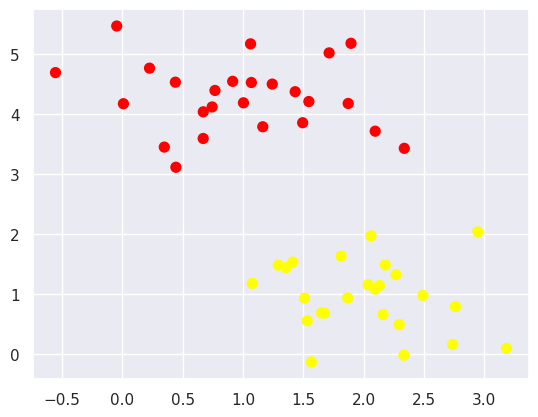
\includegraphics[width=10cm]{fig/svm_data.png}
  \caption{SVMのデータ}
  \label{fig:svm_data}
\end{figure}

赤色と黄色の2クラスのデータを分類するために,2つのクラスを分離する直線を見つけることが目標です.
このとき,どのようにして直線を引くことができるでしょうか?
次のページに進む前に\textbf{定規で試しに線を引いてみてください.}
\newpage

クラスを分割する線の例として,図\ref{fig:svm_lines}のような線が考えられます.

\begin{figure}[H]
  \centering
  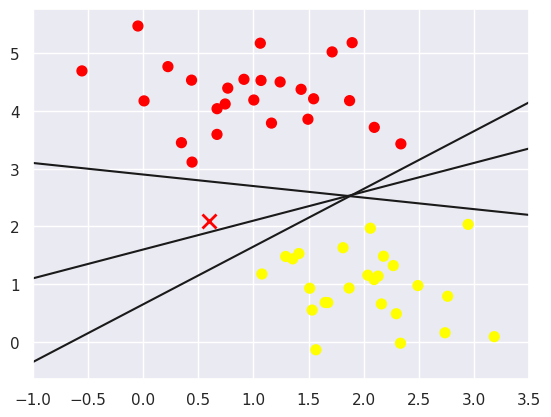
\includegraphics[width=10cm]{fig/svm_lines.png}
  \caption{SVMの直線}
  \label{fig:svm_lines}
\end{figure}

これらの線は,赤色と黄色の線をうまく分割できています.
しかしながら,どの線を境界とするかによって,図\ref{fig:svm_lines}の赤い$\times$で示したデータのクラスが変わってしまいます.
「クラス間に線を引く」という考え方は直感的で簡単ですが,実際の問題を解くためにはまだ不十分であることがわかります.

そこで登場するのが,マージン最大化という考え方です.
マージンとは,クラス間の最も近いデータ点と境界線の距離のことです.
クラス間の最も近いデータ点のことをサポートベクターと呼びます.
図\ref{fig:svm_lines}の線におけるマージンを可視化した図を図\ref{fig:svm_margin}に示します.

\begin{figure}[H]
  \centering
  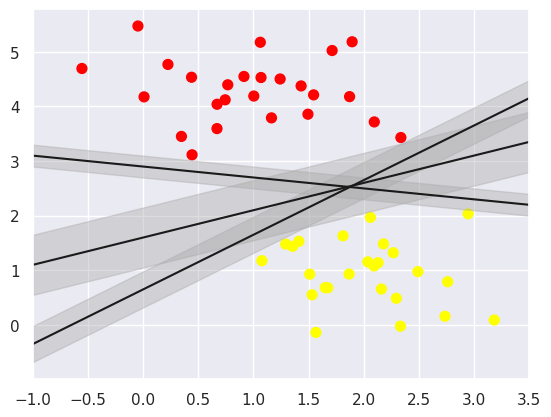
\includegraphics[width=10cm]{fig/svm_margin.png}
  \caption{SVMのマージン}
  \label{fig:svm_margin}
\end{figure}

図\ref{fig:svm_margin}の例では,中央の線が最も大きなマージンを持っています.
しかしながら,この線は最大のマージンを持っているわけではありません.
SVMでは,このようなマージンを最大化する直線を見つけることができます.
SVMによって見つけられた直線は,図\ref{fig:svm_sv}のようになります.

\begin{figure}[H]
  \centering
  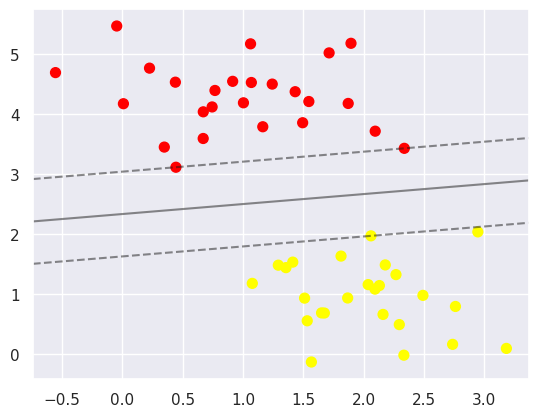
\includegraphics[width=10cm]{fig/svm_support_margin.png}
  \caption{SVMのサポートベクターとマージン}
  \label{fig:svm_sv}
\end{figure}

図\ref{fig:svm_sv}の直線は,サポートベクターによって定義されるマージンを最大化する直線です.

では,データ数が変わった場合はどうなるでしょうか?
図\ref{fig:svm_data2}に,データ数が変化した場合のSVMの分割例を示します.

\begin{figure}[H]
  \centering
  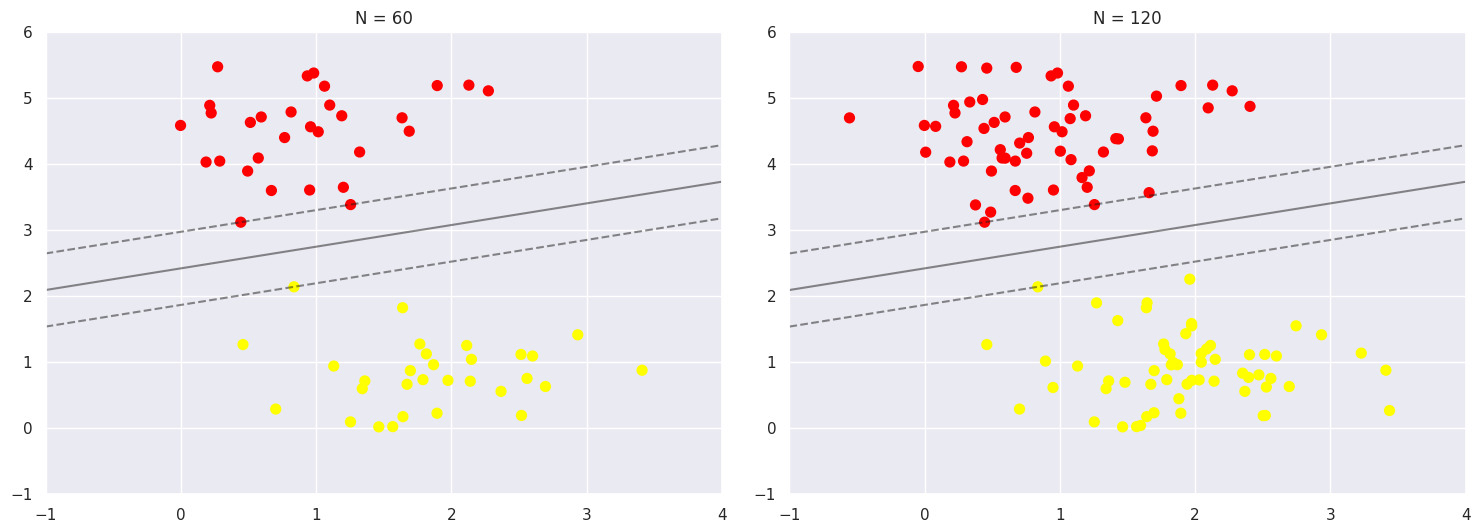
\includegraphics[height=6.1cm]{fig/svm_diff_sample_amount.png}
  \caption{データ数が変化した場合の決定境界(右:60点,左:120点)}
  \label{fig:svm_data2}
\end{figure}

SVMは境界線から遠いデータに影響されず,サポートベクターのみを用いて境界線を引いていることがわかります.
このような,境界から離れたデータに対する影響が少ない性質が,SVMの特徴の一つです.

ここまで見てきたデータは,決定境界が直線の場合のデータです.
直線で分割できるデータのことを,線形\footnote{"線形"という用語は,様々な場面で登場しますが,基本的には,直線で表せる関係を意味します.}分離可能なデータといいます.
では,境界線が直線ではない場合はどうなるでしょうか?
図\ref{fig:not_linear}に,直線で分割できないデータを示します.

\begin{figure}[H]
  \centering
  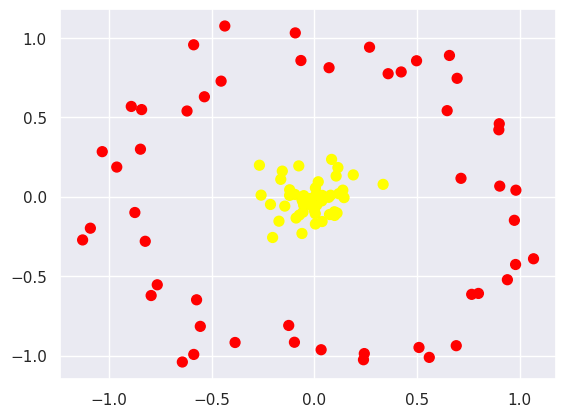
\includegraphics[width=10cm]{fig/svm_not_linear.png}
  \caption{直線で分割できないデータ}
  \label{fig:not_linear}
\end{figure}

図\ref{fig:not_linear}のデータを分割するために,図\ref{fig:not_linear}に高さ方向の次元を追加した3次元空間を考えてみましょう.
このとき,図\ref{fig:not_linear}のデータを3次元空間にプロットするための式として,次のような式が考えられます.

\begin{equation}\label{eq:kernel}
  r = e^{-(x^2 + y^2)}
\end{equation}

式(\ref{eq:kernel})は,2次元データ$(x, y)$を3次元データ$(x, y, r)$に変換する式です.
この関数は,原点が最も高い値を持ち,原点から離れるほど値が小さくなるような関数です.(図\ref{fig:RBF})
このような,距離に基づいて値が決まる関数のことを,放射基底関数(Radial Basis Function: RBF)といいます.

\begin{figure}[H]
  \centering
  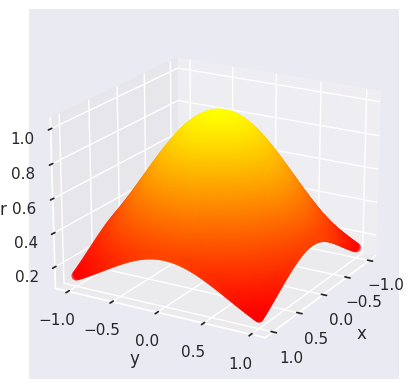
\includegraphics[width=10cm]{fig/RBF_function.png}
  \caption{RBF関数}
  \label{fig:RBF}
\end{figure}

では,RBF関数を用いて,図\ref{fig:not_linear}のデータを3次元空間にプロットしてみましょう.
図\ref{fig:3d_data}に,RBF関数を用いて3次元空間にプロットしたデータを示します.

\begin{figure}[H]
  \centering
  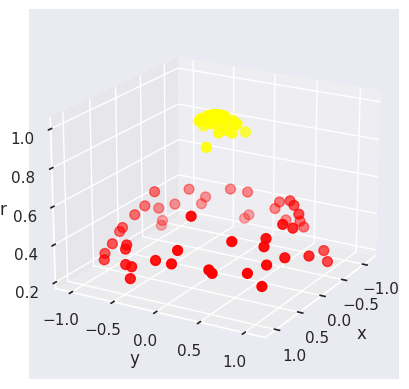
\includegraphics[width=10cm]{fig/SVM_RBF.png}
  \caption{RBF関数を用いて3次元空間にプロットしたデータ}
  \label{fig:3d_data}
\end{figure}

図\ref{fig:3d_data}を見れば,だいたい$r=0.7$となるあたりの平面で分割すればうまくいきそうだとわかります.
しかしながら,式\ref{eq:kernel}はたまたまうまくいっただけであり,(当たり前ですが)すべての場合でうまくいくわけではありません.
今回の例で考えると,RBF関数の中心をうまく設定することができなければ,データをうまく分割することができない,ということです.
詳細は割愛しますが,SVMでは,カーネルトリックという素晴らしい手法によりこの問題を解決しています.
SVMはカーネルトリックという手法の恩恵を受けている,ということだけ覚えておいてください.

話をデータの分類に戻します.図\ref{fig:svm_RBF}にRBF関数によって分類された結果を示します.

\begin{figure}[H]
  \centering
  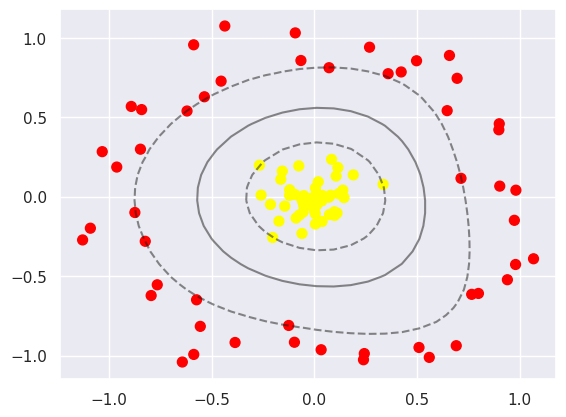
\includegraphics[width=10cm]{fig/svm_rbf_db.png}
  \caption{SVMの分類結果(RBF関数)}
  \label{fig:svm_RBF}
\end{figure}

線形に分割できなかったデータをRBF関数を用いて,マージンが最大となるようにうまく分割することができました.
RBF関数のような,データを高次元空間に写像する関数をカーネル関数といいます.
RBFカーネル以外にも,多項式カーネルやシグモイドカーネルなど,様々なカーネル関数が存在します.
カーネル関数を用いて,データを高次元空間に写像する手法のことをカーネル法といいます.
カーネル法を使用したSVMは,非線形なデータに対しても高い性能を発揮することが知られているため,頻繁に使用されます.

\section{機械学習によるデータ分類}
今週の実習では,先週の実習で皆さんから集めた手書き文字データを分類するための機械学習モデルを構築します.
現状のデータセットの状態は以下の通りです.

\begin{itemize}
  \item 取得文字: $ \bigcirc  \times $ の2文字
  \item 取得文字数: 3セット $ \times $ 10人の60文字
  \item データ長:最長のデータに合わせて引き伸ばし(M1の方で処理済)
  \item 座標軸:X, Y, Zの3軸
\end{itemize}

このデータセットを用いて,分類を行うための機械学習モデルを構築します.
\subsection{データの準備}
先週取得したデータをOneDriveからダウンロードし,Google Drive上の任意の場所にアップロードします.


\begin{center}
\textbf{\color{red}ここから後ろはまた後で書きます}
\end{center}

\section{課題}

\begin{thebibliography}{99}
  \bibitem{SVM} Jake VanderPlas. Pythonデータサイエンスハンドブック 第2版: 菊池彰訳. オライリージャパン, 2021, 545p. \\\\
\end{thebibliography}

\end{document}
